\documentclass[border={1mm 1mm 1mm 1mm},tikz,10pt]{standalone}

\usepackage{helvet}
\renewcommand{\familydefault}{\sfdefault}

\usetikzlibrary{shapes.geometric}

\usepackage{xcolor}
\definecolor{cnavy}{RGB}{4,41,112}
\definecolor{cgrey}{RGB}{72,72,72}
\definecolor{cred}{RGB}{192,0,0}
\definecolor{cgreen}{RGB}{0,157,0}

\begin{document}
	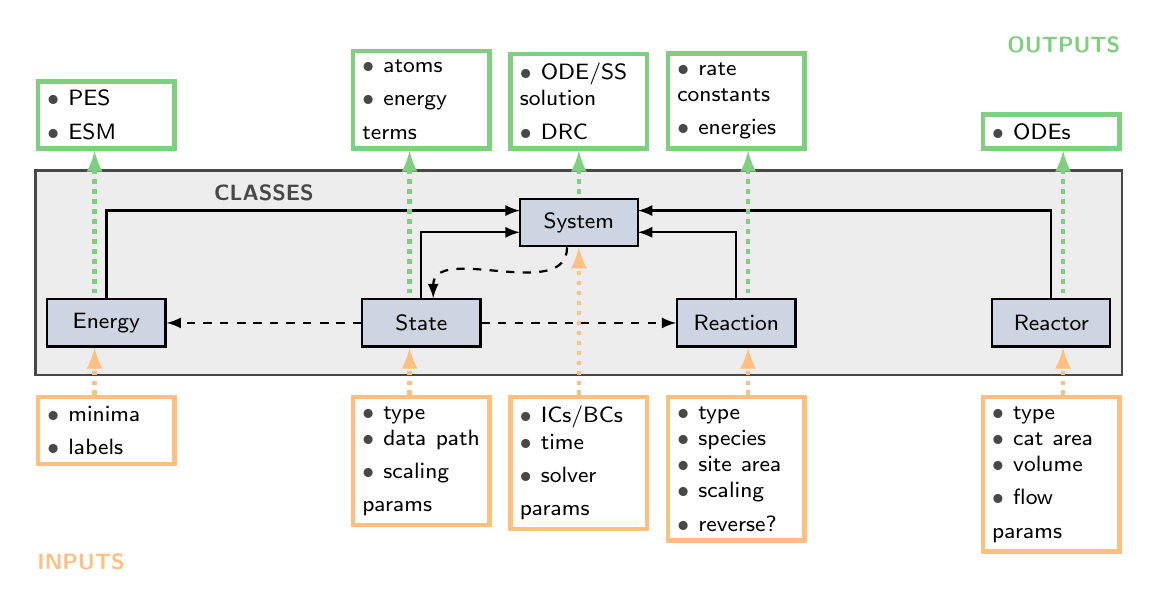
\begin{tikzpicture}[x=1cm, y=1cm, >=latex]
		\def\xleft{0}
		\def\xright{14}
		\def\ydown{0}
		\def\yup{7}
		\def\xmid{7}
		\def\ymid{3.25}
		\draw[draw=none, use as bounding box] (\xleft, \ydown) rectangle (\xright, \yup);
		\clip (\xleft-0.1, \ydown-0.1) rectangle (\xright+0.1, \yup+0.1);
		
		\def\rlen{1.5cm}
		\def\rwid{0.6cm}
		\def\blen{1.5cm}
		\def\rsep{0.85cm}
		\def\isep{0.6cm}
		\def\rupp{1.5}
		\def\bmark{\textcolor{cgrey}{$\bullet$ }}
			
		\draw[anchor=center, fill=cgrey!10, draw=cgrey, thick] ([xshift=-6.9cm, yshift=-1.1*\rwid]\xmid, \ymid) rectangle ([xshift=6.9cm, yshift=1.1*\rwid + \rupp*\rsep]\xmid, \ymid);
		
		% Classes
		\node[anchor=south] at ([xshift=-4cm, yshift=\rupp*\rsep+0.25*\rwid]\xmid, \ymid)
			{\textcolor{cgrey}{\footnotesize{\textbf{CLASSES}}}};
		\node[anchor=center, fill=cnavy!20, draw=black, thick, minimum width=\rlen, minimum height=\rwid] (system) at ([yshift=\rupp*\rsep]\xmid, \ymid)
			{\footnotesize{System}};
		\node[anchor=center, fill=cnavy!20, draw=black, thick, minimum width=\rlen, minimum height=\rwid] (energy) at ([xshift=-6cm]\xmid, \ymid)
			{\footnotesize{Energy}};
		\node[anchor=center, fill=cnavy!20, draw=black, thick, minimum width=\rlen, minimum height=\rwid] (state) at ([xshift=-2cm]\xmid, \ymid)
			{\footnotesize{State}};
		\node[anchor=center, fill=cnavy!20, draw=black, thick, minimum width=\rlen, minimum height=\rwid] (reaction) at ([xshift=2cm]\xmid, \ymid)
			{\footnotesize{Reaction}};
		\node[anchor=center, fill=cnavy!20, draw=black, thick, minimum width=\rlen, minimum height=\rwid] (reactor) at ([xshift=6cm]\xmid, \ymid)
			{\footnotesize{Reactor}};	
%		\node[anchor=west, fill=cnavy!20, draw=black, thick, minimum width=\rlen, minimum height=\rwid] (uncertainty) at ([xshift=\rsep]energy.east)
%			{Uncertainty};
	
		% Arrows
		\path[thick, ->, dashed] ([xshift=-0.1*\rlen]system.south) edge[out=270, in=90] node [left] {} ([xshift=0.1*\rlen]state.north);
		\path[thick, ->, dashed] (state.east) edge[out=0, in=180] node [left] {} (reaction.west);
		\path[thick, ->, dashed] (state.west) edge[out=180, in=0] node [left] {} (energy.east);
		\draw[thick, ->] 
			 (reaction.north) --
			 ([yshift=\rupp*\rsep-0.73*\rwid]reaction.north) -- 
			 ([xshift=-2cm+0.5*\rlen, yshift=\rupp*\rsep-0.73*\rwid]reaction.north);
		\draw[thick, ->] 
			(reactor.north) --
			([yshift=\rupp*\rsep-0.27*\rwid]reactor.north) -- 
			([xshift=-6cm+0.5*\rlen, yshift=\rupp*\rsep-0.27*\rwid]reactor.north);
		\draw[thick, ->] 
			(state.north) --
			([yshift=\rupp*\rsep-0.73*\rwid]state.north) -- 
			([xshift=2cm-0.5*\rlen, yshift=\rupp*\rsep-0.73*\rwid]state.north);
		\draw[thick, ->] 
			(energy.north) --
			([yshift=\rupp*\rsep-0.27*\rwid]energy.north) -- 
			([xshift=6cm-0.5*\rlen, yshift=\rupp*\rsep-0.27*\rwid]energy.north);	

		% Inputs
		\node[anchor=south west] at (\xleft, \ydown)
			{\textcolor{orange!50}{\footnotesize{\textbf{INPUTS}}}
		};
		\node[anchor=north, fill=white, draw=orange!50, ultra thick, text width=\blen] (Ein) at ([yshift=-1*\isep]energy.south)
			{\footnotesize{\bmark minima\\
					\bmark labels}
		};
		\node[anchor=north, fill=white, draw=orange!50, ultra thick, text width=\blen] (Sin) at ([yshift=-1*\isep]state.south)
			{\footnotesize{\bmark type\\
			\bmark data path\\
			\bmark scaling params}
		};
		\node[anchor=north, fill=white, draw=orange!50, ultra thick, text width=\blen] (Rin) at ([yshift=-1*\isep]reaction.south)
			{\footnotesize{\bmark type\\
			\bmark species\\
			\bmark site area\\
			\bmark scaling\\
			\bmark reverse?}
		};
		\node[anchor=north, fill=white, draw=orange!50, ultra thick, text width=\blen] (Rein) at ([yshift=-1*\isep]reactor.south)
			{\footnotesize{\bmark type\\
			\bmark cat area\\
			\bmark volume\\
			\bmark flow params}
		};
		\node[anchor=north, fill=white, draw=orange!50, ultra thick, text width=\blen] (Syin) at ([yshift=-1*\isep-\rupp*\rsep]system.south)
			{\footnotesize{\bmark ICs/BCs\\
			\bmark time\\
			\bmark solver params}
		};

		% Input arrows
		\draw[ultra thick, ->, orange!50, opacity=1, dotted] ([xshift=-0.1*\rlen]Ein.north) -- ([xshift=-0.1*\rlen]energy.south);
		\draw[ultra thick, ->, orange!50, opacity=1, dotted] ([xshift=-0.1*\rlen]Sin.north) -- ([xshift=-0.1*\rlen]state.south);
		\draw[ultra thick, ->, orange!50, opacity=1, dotted] ([xshift=0.1*\rlen]Rin.north) -- ([xshift=0.1*\rlen]reaction.south);
		\draw[ultra thick, ->, orange!50, opacity=1, dotted] ([xshift=0.1*\rlen]Rein.north) -- ([xshift=0.1*\rlen]reactor.south);
		\draw[ultra thick, ->, orange!50, opacity=1, dotted] (Syin.north) -- (system.south);
		
		% Outputs
		\node[anchor=north east] at (\xright, \yup)
			{\textcolor{cgreen!50}{\footnotesize{\textbf{OUTPUTS}}}
		};
		\node[anchor=south, fill=white, draw=cgreen!50, ultra thick, text width=\blen] (Eout) at ([yshift=\isep+\rupp*\rsep]energy.north)
			{\footnotesize{\bmark PES\\
			\bmark ESM}
		};
		\node[anchor=south, fill=white, draw=cgreen!50, ultra thick, text width=\blen] (Sout) at ([yshift=\isep+\rupp*\rsep]state.north)
			{\footnotesize{\bmark atoms\\
			\bmark energy terms}
		};	
		\node[anchor=south, fill=white, draw=cgreen!50, ultra thick, text width=\blen] (Rout) at ([yshift=\isep+\rupp*\rsep]reaction.north)
			{\footnotesize{\bmark rate\\constants\\
			\bmark energies}
		};
		\node[anchor=south, fill=white, draw=cgreen!50, ultra thick, text width=\blen] (Reout) at ([yshift=\isep+\rupp*\rsep]reactor.north)
			{\footnotesize{\bmark ODEs}
		};
		\node[anchor=south, fill=white, draw=cgreen!50, ultra thick, text width=\blen] (Syout) at ([yshift=\isep]system.north)
			{\footnotesize{\bmark ODE/SS solution\\
			\bmark DRC}
		};
		
		% Output arrows
		\draw[ultra thick, <-, cgreen!50, opacity=1, dotted] ([xshift=-0.1*\rlen]Eout.south) -- ([xshift=-0.1*\rlen]energy.north);
		\draw[ultra thick, <-, cgreen!50, opacity=1, dotted] ([xshift=-0.1*\rlen]Sout.south) -- ([xshift=-0.1*\rlen]state.north);
		\draw[ultra thick, <-, cgreen!50, opacity=1, dotted] ([xshift=0.1*\rlen]Rout.south) -- ([xshift=0.1*\rlen]reaction.north);
		\draw[ultra thick, <-, cgreen!50, opacity=1, dotted] ([xshift=0.1*\rlen]Reout.south) -- ([xshift=0.1*\rlen]reactor.north);
		\draw[ultra thick, <-, cgreen!50, opacity=1, dotted] (Syout.south) -- (system.north);
	
	\end{tikzpicture}
\end{document}